\documentclass[11pt, a4paper]{article}
\usepackage{graphicx,wrapfig}
\usepackage[margin=2cm]{geometry}
\usepackage[acronym]{glossaries}
\usepackage[sorting=none, style=nature]{biblatex} %Imports biblatex package
\usepackage[hidelinks]{hyperref}
\usepackage{titling}
\usepackage{float}
\usepackage{caption}
\usepackage{enumitem}
\usepackage{algorithm2e}

\renewcommand{\familydefault}{\sfdefault}
\newcommand{\customcite}[2]{\mbox{
  {\small \copyright} \textit{#1} \cite{#2}}
}

\newcommand{\subtitle}[1]{%
  \posttitle{%
    \par\end{center}
    \begin{center}\LARGE#1\end{center}
    \vskip0.5em}%
}

\hypersetup{
  colorlinks   = true, %Colours links instead of ugly boxes
  urlcolor     = blue, %Colour for external hyperlinks
  linkcolor    = blue, %Colour of internal links
  citecolor   = red %Colour of citations
}

\addbibresource{references.bib} %Import the bibliography file

\makenoidxglossaries
\loadglsentries{glossary.tex}



\title{\textbf{ \\{\Huge Compte Rendu de Stage Master 2}}}
\subtitle{Galaxies Pop III, premières phases de la formation des métaux et poussières dans l'Univers à très grand Redshift (6 $<$ z $<$ ?)}
\author{Dewachter Tim}
\date{25 Mars 2024 - 28 Juin 2024}

\begin{document}

\maketitle

\newpage

\tableofcontents

\newpage

\section{Introduction}

%TODO

\subsection{Contexte}

En seulement 2 ans d'opérations, le \gls{jwst} nous a déjà ouvert de nombreuses portes jusqu'alors inaccessibles, et cela dans de nombreuses branches de l'astrophysique. Grâce à ses instruments spectroscopiques et sa sensibilité à l'infrarouge proche et moyen, il est désormais possible de sonder l'univers comme jamais auparavant. Parmi les nombreux objectifs que l'on souhaite accomplir avec ce télescope, l'un d'eux est l'étude de la formation des galaxies, de l'apparition des métaux au sein de celles-ci, et de la recherche des hypothétiques galaxies de Population III, constituées d'étoiles de métallicité nulle, formées par le gaz primordial d'Hydrogène et d'Hélium.

Ce nouvel horizon sur l'univers lointain nous permet de remonter l'histoire de l'univers comme jamais auparavant. \cite{2023arXiv230600953M} %TODO



\section{Méthodologie}

\subsection{JWST et NIRSpec}

Le \gls{jwst} est un télescope spatial de 6.5 mètres de diamètre équivalent, en orbite autour du point de Lagrange L2, et actif depuis juillet 2022 \cite{jwst_website}. Sa sensibilité dans l'infrarouge en fait un outil remarquable pour observer l'univers jeune. En effet, de par l'expansion de l'univers, la lumière des objets lointains se retrouve décalée vers le rouge : il s'agit du redshift $z$, défini comme 

\begin{equation}
    1 + z = \frac{\lambda_{obs}}{\lambda_{rest}}
\end{equation}

Avec $\lambda_{obs}$ la longueur d'onde observée, et $\lambda_{rest}$ la longueur d'onde dans le référentiel de la source (au repos). Ainsi, regarder loin dans l'espace est équivalent à regarder loin dans le passé et nécessite d'observer à des longueurs d'ondes de plus en plus grandes.

\begin{figure}[H]
  \centering
  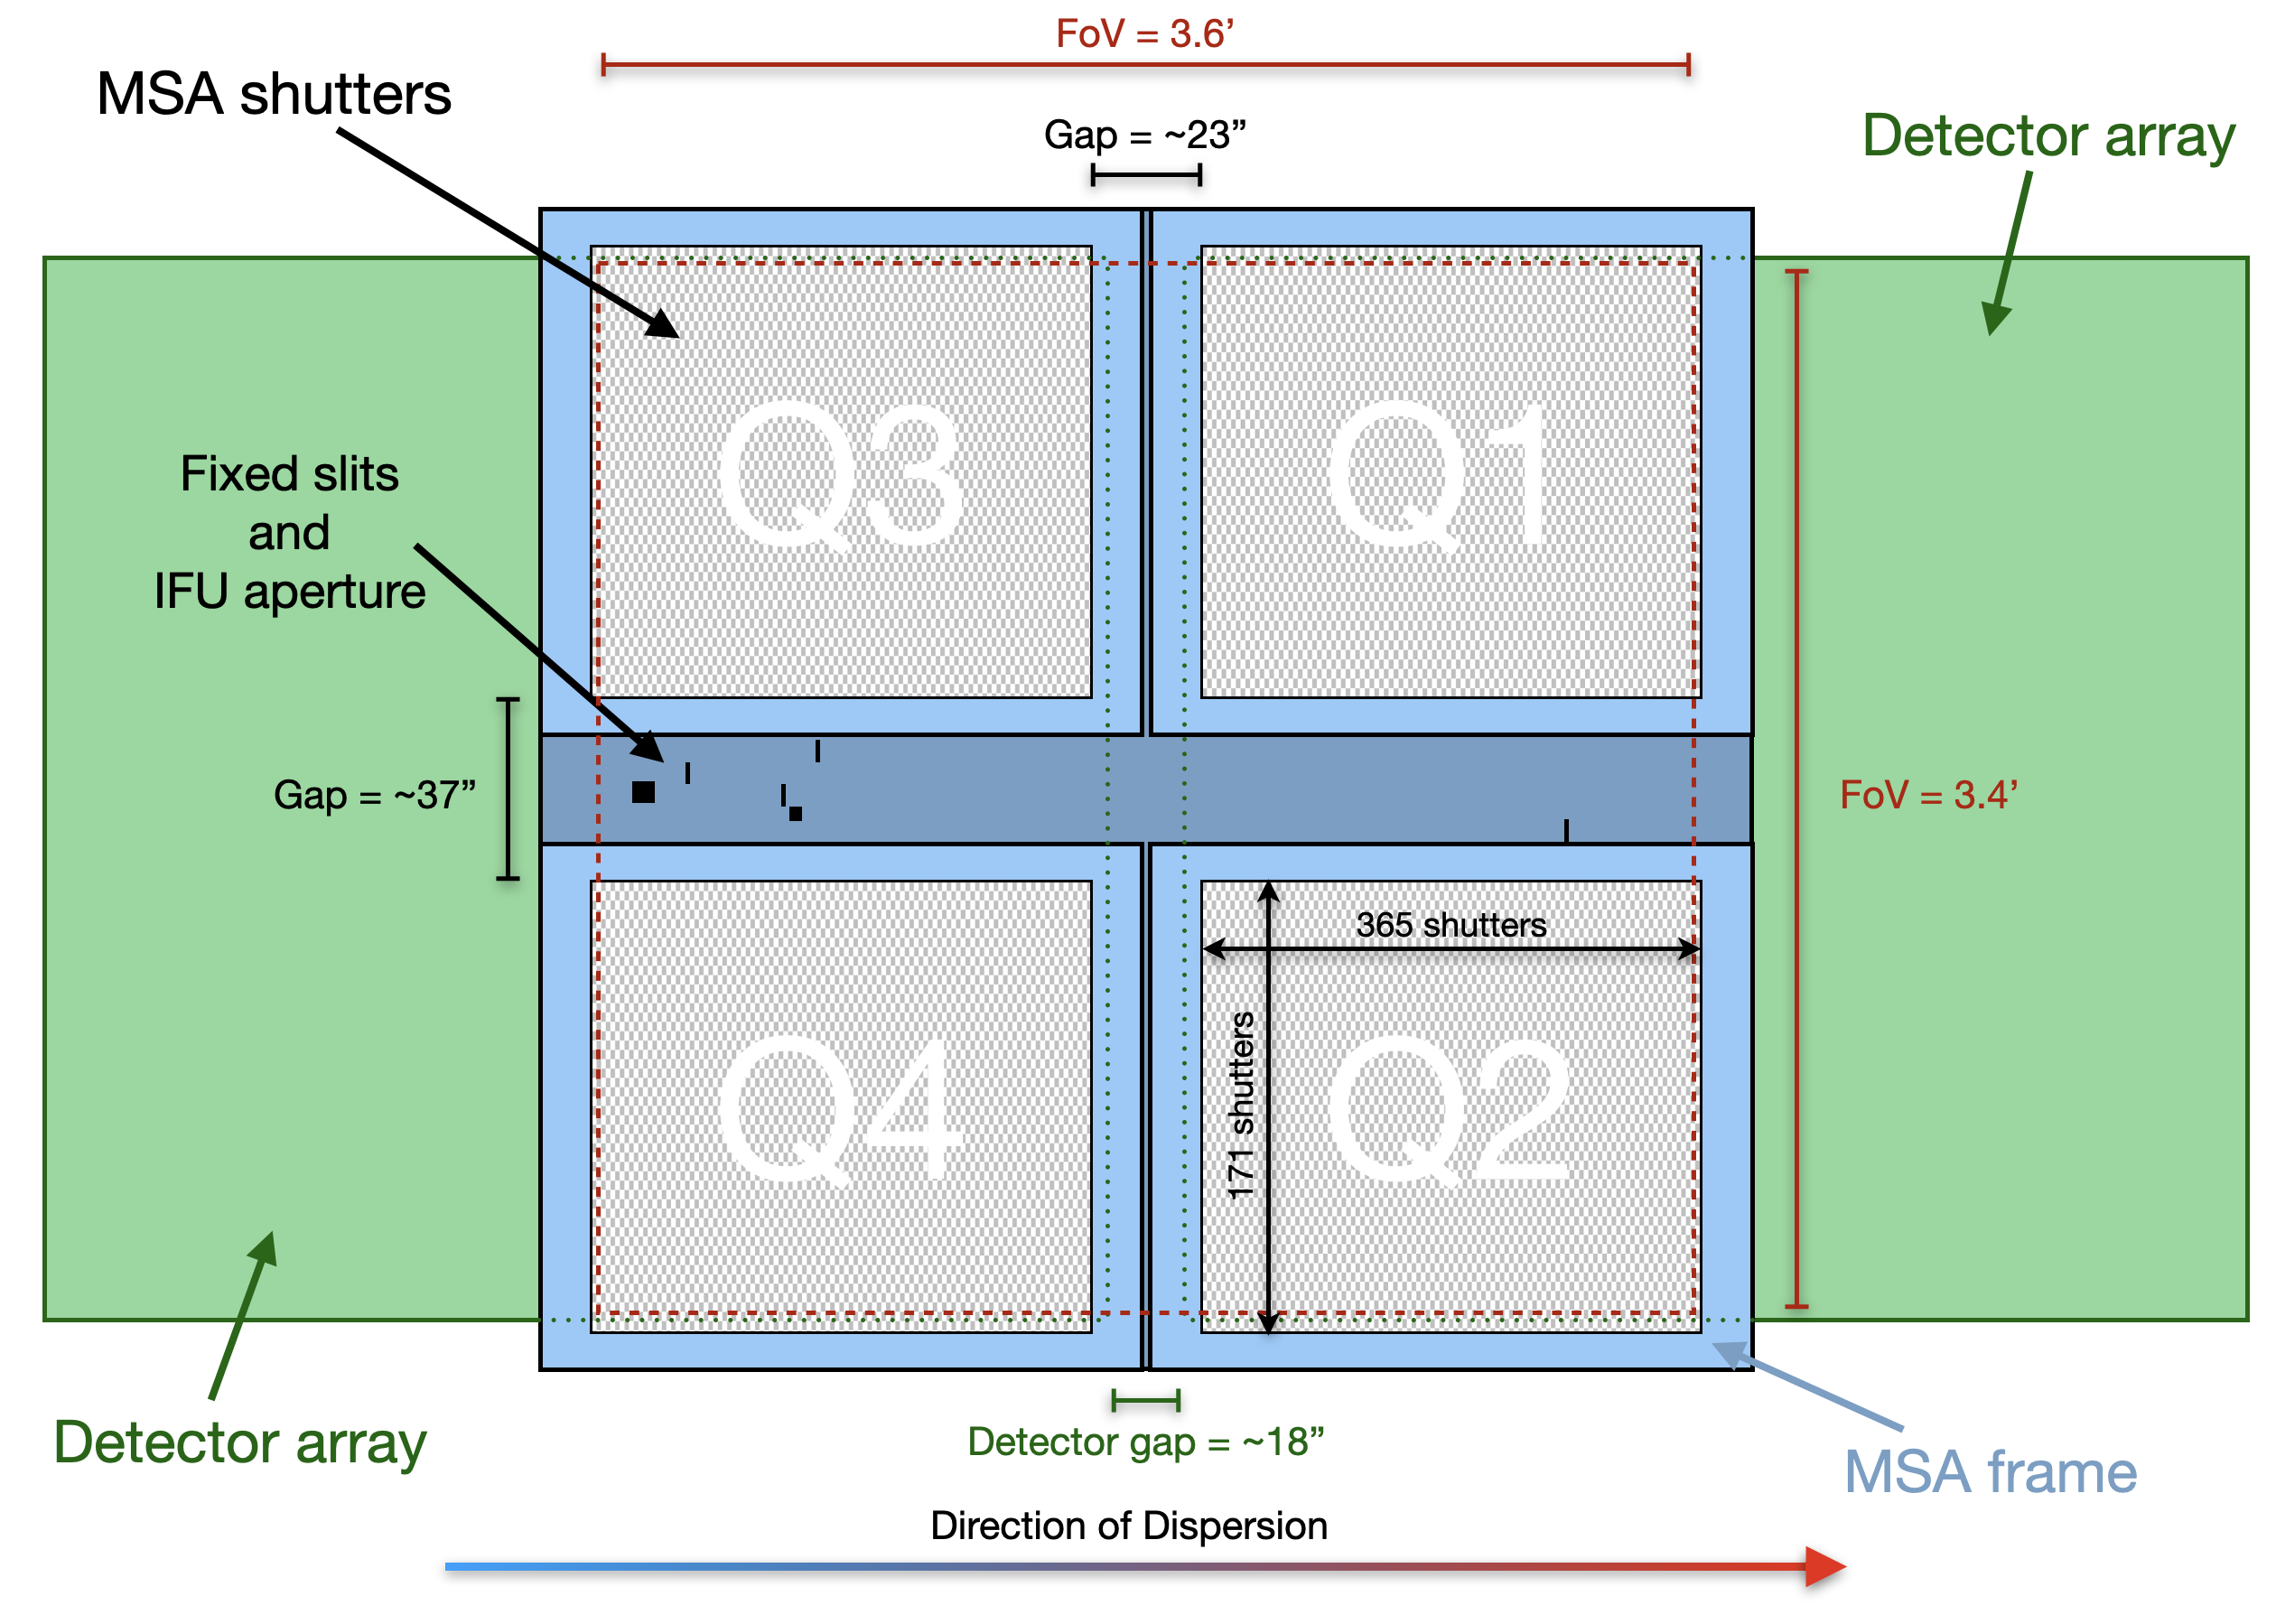
\includegraphics[scale=0.25]{assets/msa_ds_new.png}
  \caption{Disposition de MSA dans le plan focal de NIRSpec. \customcite{Ferruit et al.}{2022A&A...661A..81F}}
  \label{fig:msa_shutter}
\end{figure}

Parmi les instruments du \gls{jwst}, le \gls{nirspec} est un spectromètre sur la bande 0.6 - 5.3  µm, disposant de 3 modes de résolution : prism ($R \sim 100$), medium grating ($R \sim 1000$), high grating ($R \sim 2700$) \cite{nirspec}. L'un des atouts principaux de \gls{nirspec} est son \gls{msa}, une grille de près de 250 000 obturateurs, couvrant une surface de 3.6' x 3.4' sur le ciel, chacun pouvant être individuellement ouvert ou fermé \cite{msa} (voir \ref{fig:msa_shutter}). Ceci permet d'observer dans le mode \gls{mos} de \gls{nirspec}. Comme son nom l'indique, la spectroscopie multi-objet permet d'étudier le spectre de plusieurs objets dans un même champ, mais la grille d'obturateurs apporte également un outil fondamental dans l'extraction des spectres : la soustraction du fond.

\subsection{Fond, Nodding et Slitlet}

Lorsqu'on s'intéresse à des sources de faible brillance, le flux lumineux mesuré peut rapidement se trouver dominer par les émissions du fond. Que ce soit le fond diffus infrarouge, produit par des sources extragalactiques non résolues, la lumière zodiacale, produite par la poussière interplanétaire, le rayonnement de la Voie Lactée ou l'émission thermique du JWST lui-même, l'infrarouge est un domaine facilement parasité par des signaux indésirables \cite{jwst_background}. De plus, la nature de ses composantes fait de ce fond un signal anisotrope. Il n'est donc pas si simple d'en établir un modèle universel à soustraire de façon systématique. On a la mesure du fond en fonction de la longueur d'onde ci dessous \ref{fig:background_jwst} : 

\begin{figure}[H]
  \centering
  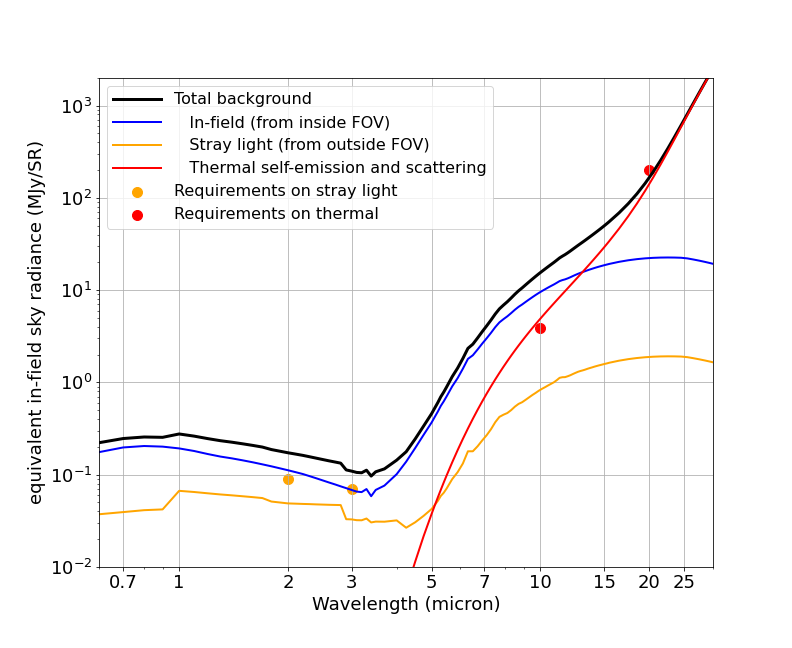
\includegraphics[scale=0.4]{assets/background_jwst.png}
  \caption{Flux par unité d'angle solide reçu par le JWST en fonction de la longueur d'onde. On remarque qu'à mesure que $\lambda$ augmente, l'émission thermique du télescope domine. \customcite{STScI}{jwst_background}}
  \label{fig:background_jwst}
\end{figure}


Cependant, il reste tout de même envisageable de corriger ce signal parasite. En effet, en ouvrant les obturateurs à proximité de celui imageant la source, il devient possible d'extraire le fond localement autour de la source, que l'on peut alors soustraire au spectre de cette dernière.

La configuration habituelle consiste en l'ouverture de 3 obturateurs dans la direction perpendiculaire à la direction de dispersion, on parlera par la suite de \textit{Slitlet}. On réalise alors 3 expositions, chacune en orientant le télescope de façon à avoir la source dans un obturateur différent : il s'agit du nodding. Ce mouvement entre chaque exposition offre également un autre avantage au travers du \textit{dithering}. La \gls{psf} de \gls{nirspec} est effectivement de $0.08 ''$ à $\lambda = 2.46 \mu m$ \cite{10_1051_0004_6361_202142663}. 
Comme $PSF \propto \lambda$, on a une \gls{psf} variant de $0.02 ''$ à $0.17''$ le long de la plage de longueur d'onde observable. Comme la taille d'un pixel est $\sim 0.1''$ dans la direction spatiale, la \gls{psf} est sous échantillonnée presque partout. Le dithering permet alors d'améliorer cet échantillonnage par des corrections sub-pixels, mais également de s'affranchir des éventuels pixels défectueux ou des rayons cosmiques.

On résume ceci dans la figure \ref{fig:msa_slitlet}.


\begin{figure}[H]
  \centering
  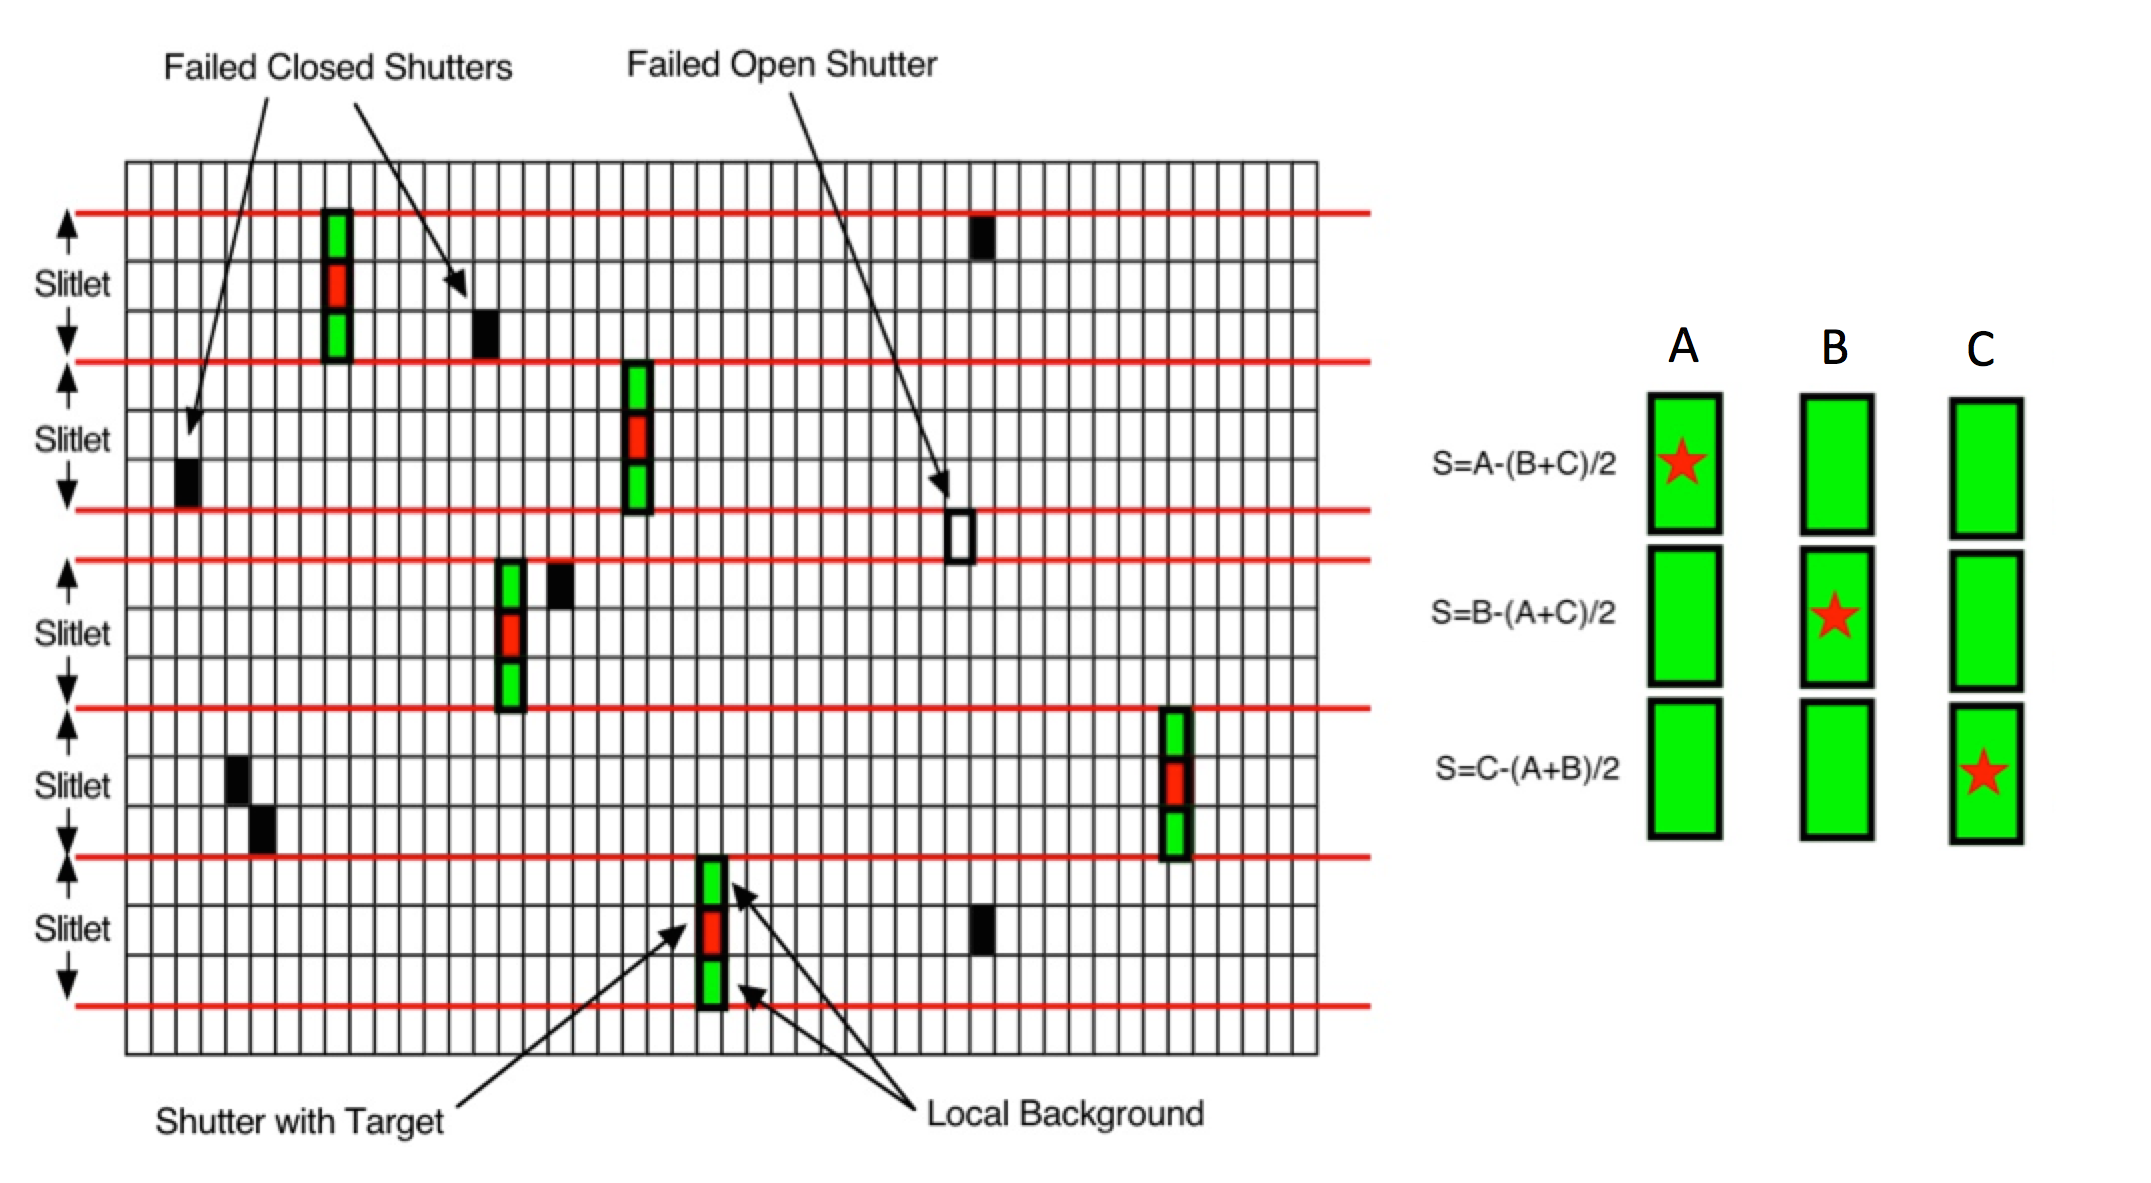
\includegraphics[scale=0.2]{assets/MSA_sky_strategy.png}
  \caption{Schéma de MSA et de slitlets. On réalise des séries de 3 images, chacune ayant la source dans un obturateur différent, et on utilise les 2 obturateurs restant pour déterminer le spectre du fond. \customcite{NIRSpec Instrument Development Team}{mos}}
  \label{fig:msa_slitlet}
\end{figure}

\subsection{Le pipeline JWST}

Le code permettant de traiter les données reçues du JWST, appelé pipeline (figure \ref{fig:jwst_pipeline}), se décompose en 3 grandes étapes, celles ci étant de plus en plus spécifique aux types de données que l'on cherche à étudier à mesure que l'on progresse dans le pipeline.

Ainsi, dans notre cas, les 3 étapes sont telles que :\\


\begin{minipage}{.45\linewidth}
  \begin{itemize}[left=0cm]
    \item \textbf{Detector 1} : Applique les corrections au niveau du détecteur, tel que le masquage des pixels morts/chauds et des rayons cosmiques, la linéarisation du nombre d'\gls{adu}, la suppression du biais et du courant d'obscurité... Cette étape est la même pour tous les instruments du \gls{jwst}.
    \item \textbf{Spectroscopy 2} : Applique des modifications optiques, telles que la correction de champ plat et des pertes de lumières liées aux barres séparant les obturateurs, mais calibre également la photométrie et les données \gls{wcs}, associant à chaque pixel des coordonnées spatiales et spectrales. C'est ici que les images de chaque slitlets sont extraites de l'image initiale et que la soustraction du fond s'applique.
    \item \textbf{Spectroscopy 3} : Combine plusieurs expositions entre elles, appliquant ainsi le dithering / nodding discuté plus tôt, ré-échantillonne les images 2D et extrait les spectres 1D de celles-ci.
  \end{itemize}
  \end{minipage}
  \hfill
  \begin{minipage}{.5\linewidth}
  \centering
  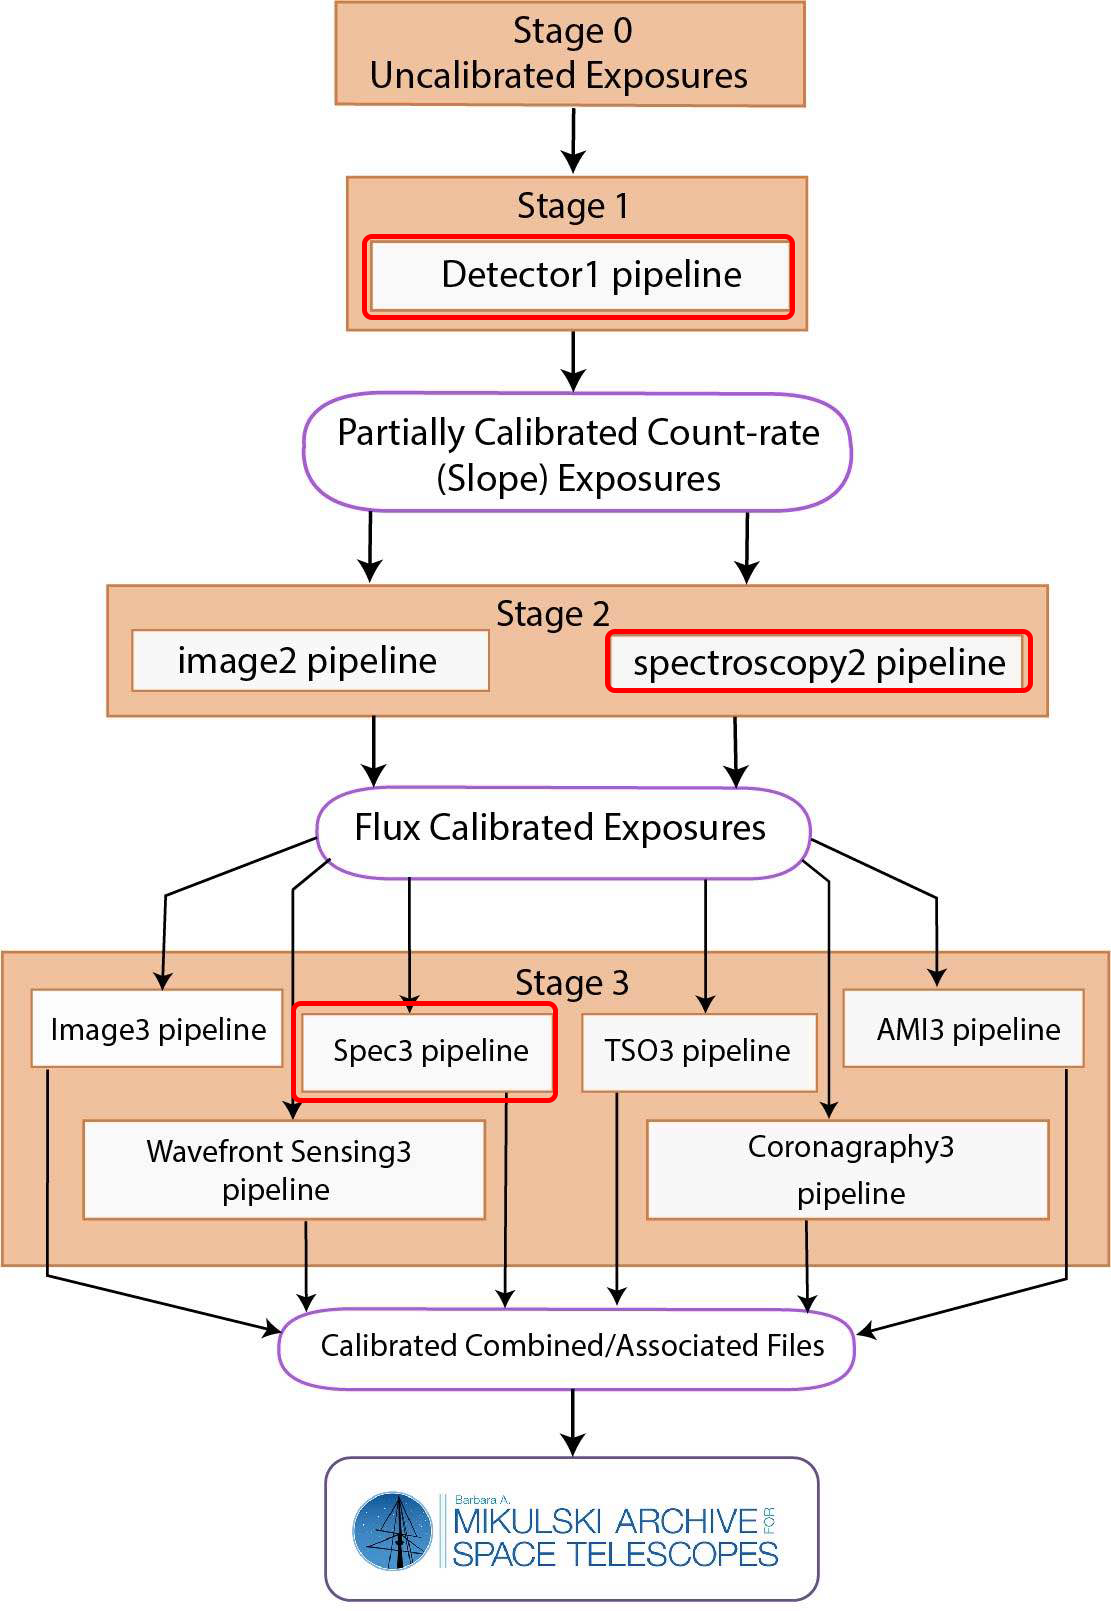
\includegraphics[scale=0.15]{assets/jwst_pipeline.jpg}
  \captionof{figure}{Schéma des différentes étapes du pipeline. Les étapes adaptées à nos données sont encadrées en rouge.\customcite{STScI}{jwst_pipeline}}
  \label{fig:jwst_pipeline}
  \end{minipage}

  \subsubsection{Soustraction du fond par défaut}

  Dans le cas de données \gls{nirspec} \gls{mos}, la soustraction du fond se fait pixel par pixel, lors de l'étape 2 du pipeline. Sur chaque slitlet, pour une exposition donnée, on considère les 2 expositions restantes comme du signal de fond, on les moyenne donc avant de les soustraire à l'image initiale. Cette étape est décrite sur la figure \ref{fig:msa_slitlet}

  Cette méthode a l'avantage majeur de permettre de soustraire le fond localement autour de la source. Cependant, celle ci se heurte à un problème dans le cas où la source est suffisamment étendue pour être visible depuis un des obturateurs de fond, ou dans celui où celle ci est mal centrée dans l'obturateur principal, mais également dans la situation plus intéressante où une autre source suffisamment brillante se situe dans le champ d'un des obturateurs de fond. Dans chacun de ces scénarios, le spectre de "fond" n'en est plus réellement un : on observe une sur-correction du spectre de l'objet. Les raies d'émission sont atténuées sur la bande de signal et des raies inversées apparaissent sur les autres bandes, en raison de la soustraction. C'est ce que l'on observe sur la figure \ref{fig:negative_trace} : les bandes au-dessus et en dessous de la bande principale présentent un spectre négatif. Cette sur-correction a également pour conséquence de cacher toute galaxie de faible luminosité se trouvant dans une des bandes du fond.\\
  
  \begin{figure}[H]
    \centering
    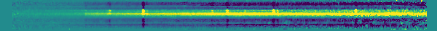
\includegraphics[scale=1.1]{assets/negative_trace_nirspec.png}
    \caption{Exemple d'une image 2D d'un spectre de \gls{nirspec} en fin de traitement classique. On observe clairement des spectres négatifs au-dessus et en dessous de la bande contenant le signal. Ceci est particulièrement visible à proximité des raies intenses. \customcite{jw01345-o063\_s03939\_nirspec\_clear-prism\_s2d}{portal_mast}}
    \label{fig:negative_trace}
  \end{figure}

  Le pipeline offre également un autre algorithme, dit de master background, qui extrait puis combine les spectres de plusieurs obturateurs de fond, ailleurs dans le champ, avant de ré-interpoler le spectre en 2D et de le soustraire. Cette méthode, bien qu'offrant en général un meilleur rapport signal sur bruit, a le désavantage de perdre l'aspect local du fond avec la soustraction pixel par pixel.

  \subsubsection{Soustraction du fond personnalisée}

  Nous allons ici chercher à établir une nouvelle méthode de soustraction du fond, combinant le meilleur signal sur bruit du master background avec la composante locale de la soustraction pixel par pixel. L'algorithme est comme suit :\\

  \begin{algorithm}
    $raw$ = données à traiter \;
    Appliquer le stage 1 du pipeline sur $raw$ \;
    Appliquer le stage 2 du pipeline sur $raw$ jusqu'à l'étape Master Background \;
    Application temporaire des étapes FlatField, PathLoss, BarShadow, Photom, ResampleSpec \;
    \ForEach{Slitlet dans $raw$}{
      \If{Nombre de shutters dans slitlet = 3}{
        Moyenne spectrale de l'image dans la direction de dispersion \;
        Détermination des positions $y_i$ de chaque bande par ajustement de 3 profils gaussien \;
        \ForEach{$i \in [1,2,3] \; \& \; i \neq source$}{
          Extraction et moyenne spatiale des $z_j^i$, les 2 bandes de fond, centrée sur $y_i$, avec une étendue spatiale de 3 pixels \;
          Extraction et moyenne spatiale des $\lambda_j^i$, longueurs d'ondes associées \;
          Extraction et moyenne spatiale des $(\sigma_j^i)^2$, les variances sur $z_j^i$ associées \;          
         }
        Ajuster une spline $f(\lambda_j^i)$ aux données $z_j^i$, de degré $k=5$ et de facteur de lissage $s=0.01$ \;
        Créer une nouvelle image $Z_{(x,y)} = f(\lambda_{(x,y)})$ \;
        Appliquer les étapes inverses de ResampleSpec, Photom, BarShadow, PathLoss, FlatField \;
        Calcul des données traitées $trait\acute{e}e_{(x,y)} = raw_{(x,y)} - Z_{(x,y)}$ \;
        }
    }
    Appliquer les étapes suivantes du stage 2 du pipeline sur $raw$\;
    Appliquer le stage 3 du pipeline sur $raw$\;
  \end{algorithm}









\printnoidxglossaries

\printbibliography %Prints bibliography


\end{document}
